%%%%%%%%%%%%%%%%%%%%%%%%%%%%%%%%%%%%%%%%%
% University Assignment Title Page 
% LaTeX Template
% Version 1.0 (27/12/12)
%
% This template has been downloaded from:
% http://www.LaTeXTemplates.com
%
% Original author:
% WikiBooks (http://en.wikibooks.org/wiki/LaTeX/Title_Creation)
%
% License:
% CC BY-NC-SA 3.0 (http://creativecommons.org/licenses/by-nc-sa/3.0/)
% 
% Instructions for using this template:
% This title page is capable of being compiled as is. This is not useful for 
% including it in another document. To do this, you have two options: 
%
% 1) Copy/paste everything between \begin{document} and \end{document} 
% starting at \begin{titlepage} and paste this into another LaTeX file where you 
% want your title page.
% OR
% 2) Remove everything outside the \begin{titlepage} and \end{titlepage} and 
% move this file to the same directory as the LaTeX file you wish to add it to. 
% Then add \input{./title_page_1.tex} to your LaTeX file where you want your
% title page.
%
%%%%%%%%%%%%%%%%%%%%%%%%%%%%%%%%%%%%%%%%%
%\title{Title page with logo}
%----------------------------------------------------------------------------------------
%	PACKAGES AND OTHER DOCUMENT CONFIGURATIONS
%----------------------------------------------------------------------------------------

\documentclass[12pt]{article}
\usepackage[spanish]{babel}
\selectlanguage{spanish}
\usepackage[utf8]{inputenc}
\usepackage{amsmath}
\usepackage[hidelinks]{hyperref}
\usepackage{graphicx}
\usepackage{tabularx}

%Para centrar imagenes
\usepackage[export]{adjustbox}
\usepackage[colorinlistoftodos]{todonotes}

\usepackage{xcolor,colortbl}
\definecolor{Gray}{gray}{0.85}
\newcolumntype{a}{>{\columncolor{Gray}}l}

\usepackage{pdflscape}
\usepackage[final]{pdfpages}
\usepackage{svg}
\usepackage{float}
\usepackage{changepage}

%Codigo SQL
\usepackage{listings}
\usepackage{color}

\definecolor{mygreen}{rgb}{0,0.6,0}
\definecolor{mygray}{rgb}{0.5,0.5,0.5}
\definecolor{mymauve}{rgb}{0.58,0,0.82}

\lstset{ %
	backgroundcolor=\color{white},   % choose the background color; you must add \usepackage{color} or \usepackage{xcolor}; should come as last argument
	basicstyle=\ttfamily\tiny,        % the size of the fonts that are used for the code
	breakatwhitespace=false,         % sets if automatic breaks should only happen at whitespace
	breaklines=true,                 % sets automatic line breaking
	captionpos=b,                    % sets the caption-position to bottom
	commentstyle=\color{mygreen},    % comment style
	deletekeywords={...},            % if you want to delete keywords from the given language
	escapeinside={\%*}{*)},          % if you want to add LaTeX within your code
	extendedchars=true,              % lets you use non-ASCII characters; for 8-bits encodings only, does not work with UTF-8
	frame=single,	                   % adds a frame around the code
	keepspaces=true,                 % keeps spaces in text, useful for keeping indentation of code (possibly needs columns=flexible)
	keywordstyle=\color{blue},       % keyword style
	language=SQL,                 % the language of the code
	morekeywords={*,...},           % if you want to add more keywords to the set
	numbers=left,                    % where to put the line-numbers; possible values are (none, left, right)
	numbersep=5pt,                   % how far the line-numbers are from the code
	numberstyle=\tiny\color{mygray}, % the style that is used for the line-numbers
	rulecolor=\color{black},         % if not set, the frame-color may be changed on line-breaks within not-black text (e.g. comments (green here))
	showspaces=false,                % show spaces everywhere adding particular underscores; it overrides 'showstringspaces'
	showstringspaces=false,          % underline spaces within strings only
	showtabs=false,                  % show tabs within strings adding particular underscores
	stepnumber=2,                    % the step between two line-numbers. If it's 1, each line will be numbered
	stringstyle=\color{mymauve},     % string literal style
	tabsize=2,	                   % sets default tabsize to 2 spaces
	title=\lstname                   % show the filename of files included with \lstinputlisting; also try caption instead of title
}


\newcommand{\requisito}[3]{\begin{itemize}
		\item \textbf{Como} #1 \item \textbf{Quiero} #2 \item \textbf{Para} #3
	\end{itemize}}

\newcommand{\requit}[5]{\hrulefill \newline \textbf{#1} - #2 \requisito{#3}{#4}{#5}}

\newcommand{\prueba}[3]{\begin{itemize}
		\item \textbf{Como} #1 \item \textbf{Quiero} #2 \item \textbf{Para} #3
\end{itemize}}

\begin{document}

\begin{titlepage}

\newcommand{\HRule}{\rule{\linewidth}{0.5mm}} % Defines a new command for the horizontal lines, change thickness here

\center % Center everything on the page
 
%----------------------------------------------------------------------------------------
%	HEADING SECTIONS
%----------------------------------------------------------------------------------------

\textsc{\LARGE Universidad de Sevilla}\\[1.5cm] % Name of your university/college
\textsc{\Large IISSI}\\[0.5cm] % Major heading such as course name
\textsc{\large Proyecto}\\[0.5cm] % Minor heading such as course title

%----------------------------------------------------------------------------------------
%	TITLE SECTION
%----------------------------------------------------------------------------------------

\HRule \\[0.4cm]
{ \huge \bfseries Modas Omaita}\\[0.4cm] % Title of your document
\HRule \\[1.5cm]
 
%----------------------------------------------------------------------------------------
%	AUTHOR SECTION
%----------------------------------------------------------------------------------------
\begin{minipage}{0.5\textwidth}
\large
\emph{Autores:}\\
Daniel González Corzo\\
Jesús Pineda Márquez\\
José Luis Mármol Romero \\
Roberto Hueso Gómez
\end{minipage}

% If you don't want a supervisor, uncomment the two lines below and remove the section above
%\Large \emph{Author:}\\
%John \textsc{Smith}\\[3cm] % Your name

%----------------------------------------------------------------------------------------
%	DATE SECTION
%----------------------------------------------------------------------------------------
\vspace{1cm}
{\large \today}\\[1cm] % Date, change the \today to a set date if you want to be precise

%----------------------------------------------------------------------------------------
%	LOGO SECTION
%----------------------------------------------------------------------------------------


\includegraphics[width=7cm]{logo-US.png} % Include a department/university logo - this will require the graphicx package
 
%----------------------------------------------------------------------------------------

\vfill % Fill the rest of the page with whitespace

\end{titlepage}

\tableofcontents
\newpage

\section{Introducción}

Omaita Modas es una tienda situada en la localidad de Alcalá de Guadaira y más exactamente en la calle Pepe Luces nº20, la cual pertenece a una cadena de tiendas de ropa que se especializa en la venta de ropa y accesorios a un público maduro y femenino.
Nuestro cliente busca ser una tienda puntera en su cadena gracias a que tiene a su disposición toda la atención del público de la localidad, ya que es la única de esta cadena en la misma. Actualmente nuestro cliente no pasa por la mejor situación en lo que a clientela se refiere, además de que carece de personal, por tanto, nuestro proyecto tiene como base ayudar a nuestro cliente en la gestión de la tienda con un sistema informático, el cual nos permita realizar pedidos a proveedores y visualizar productos en el stock de la otras tiendas de la cadena,  y la creación de una página online donde sus clientes puedan visualizar y comprar un producto determinado en cualquier momento, con esto último se quiere conseguir ampliar la clientela de la tienda.
\\\\
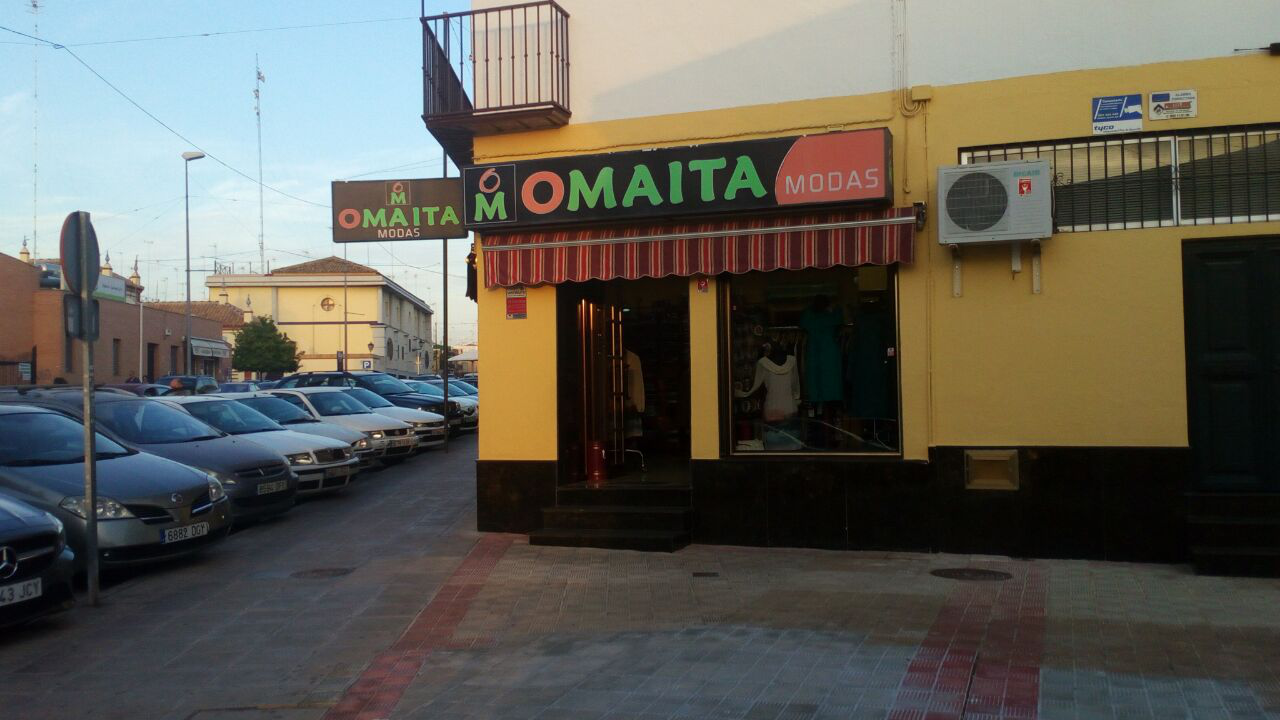
\includegraphics[width=\textwidth, center]{images/tienda1.jpg}

\section{Glosario de Términos}
\begin{table}
	\centering
	\begin{tabularx}{\textwidth}{|l|X|}
		\hline \rowcolor{Gray}
		Término & Descripción \\
		\hline
		Albarán de entrega & Documento obtenido en la recepción del pedido que verifica la correcta entrega del mismo.\\ \hline
		Almacén & Almacén que tienen en común todas las tiendas de la cadena Omaita modas.\\ \hline
		Aviso & Notificación o anuncio dado para comunicar de la falta o limitación. \\ \hline
		Consulta & Actividad que se realiza para tratar de encontrar cualquier entidad almacenada en la base de datos. \\ \hline
		Cadena & Conjunto de tiendas relacionadas entre sí que ofrecen una mezcla estándar de productos, las cuales disponen de almacenes en común. \\ \hline
		Categoría & Tipo de producto que hay en la tienda. \\ \hline
		Emplazamiento & Inmueble de la cadena, puede ser una tienda o el almacén \\ \hline
		Factura & Documento en el que se plasman las compras realizadas además del número de referencia en la base de datos a la lista de compras.\\ \hline
		Pedido & Petición de productos de un emplazamiento al proveedor. \\ \hline
		Proveedor & Entidad económica a la cual varias empresas le compran el material que usarán en la misma o que luego lo venderán al por menor. \\ \hline
		Solicitud & Petición de traspaso de un emplazamiento a otro \\ \hline
		Stock & Conjunto de mercancías o productos que se tienen almacenados en espera de su venta o comercialización. \\ \hline
		Stock mínimo & 5 unidades de un producto almacenadas \\ \hline
		Traspaso & Transferencia de uno o varios productos de un emplazamiento a otro \\ \hline
	\end{tabularx}
\end{table}

\begin{landscape}
\section{Modelo de negocio}

\subsection{Proceso de venta}
\begin{figure}[H]
	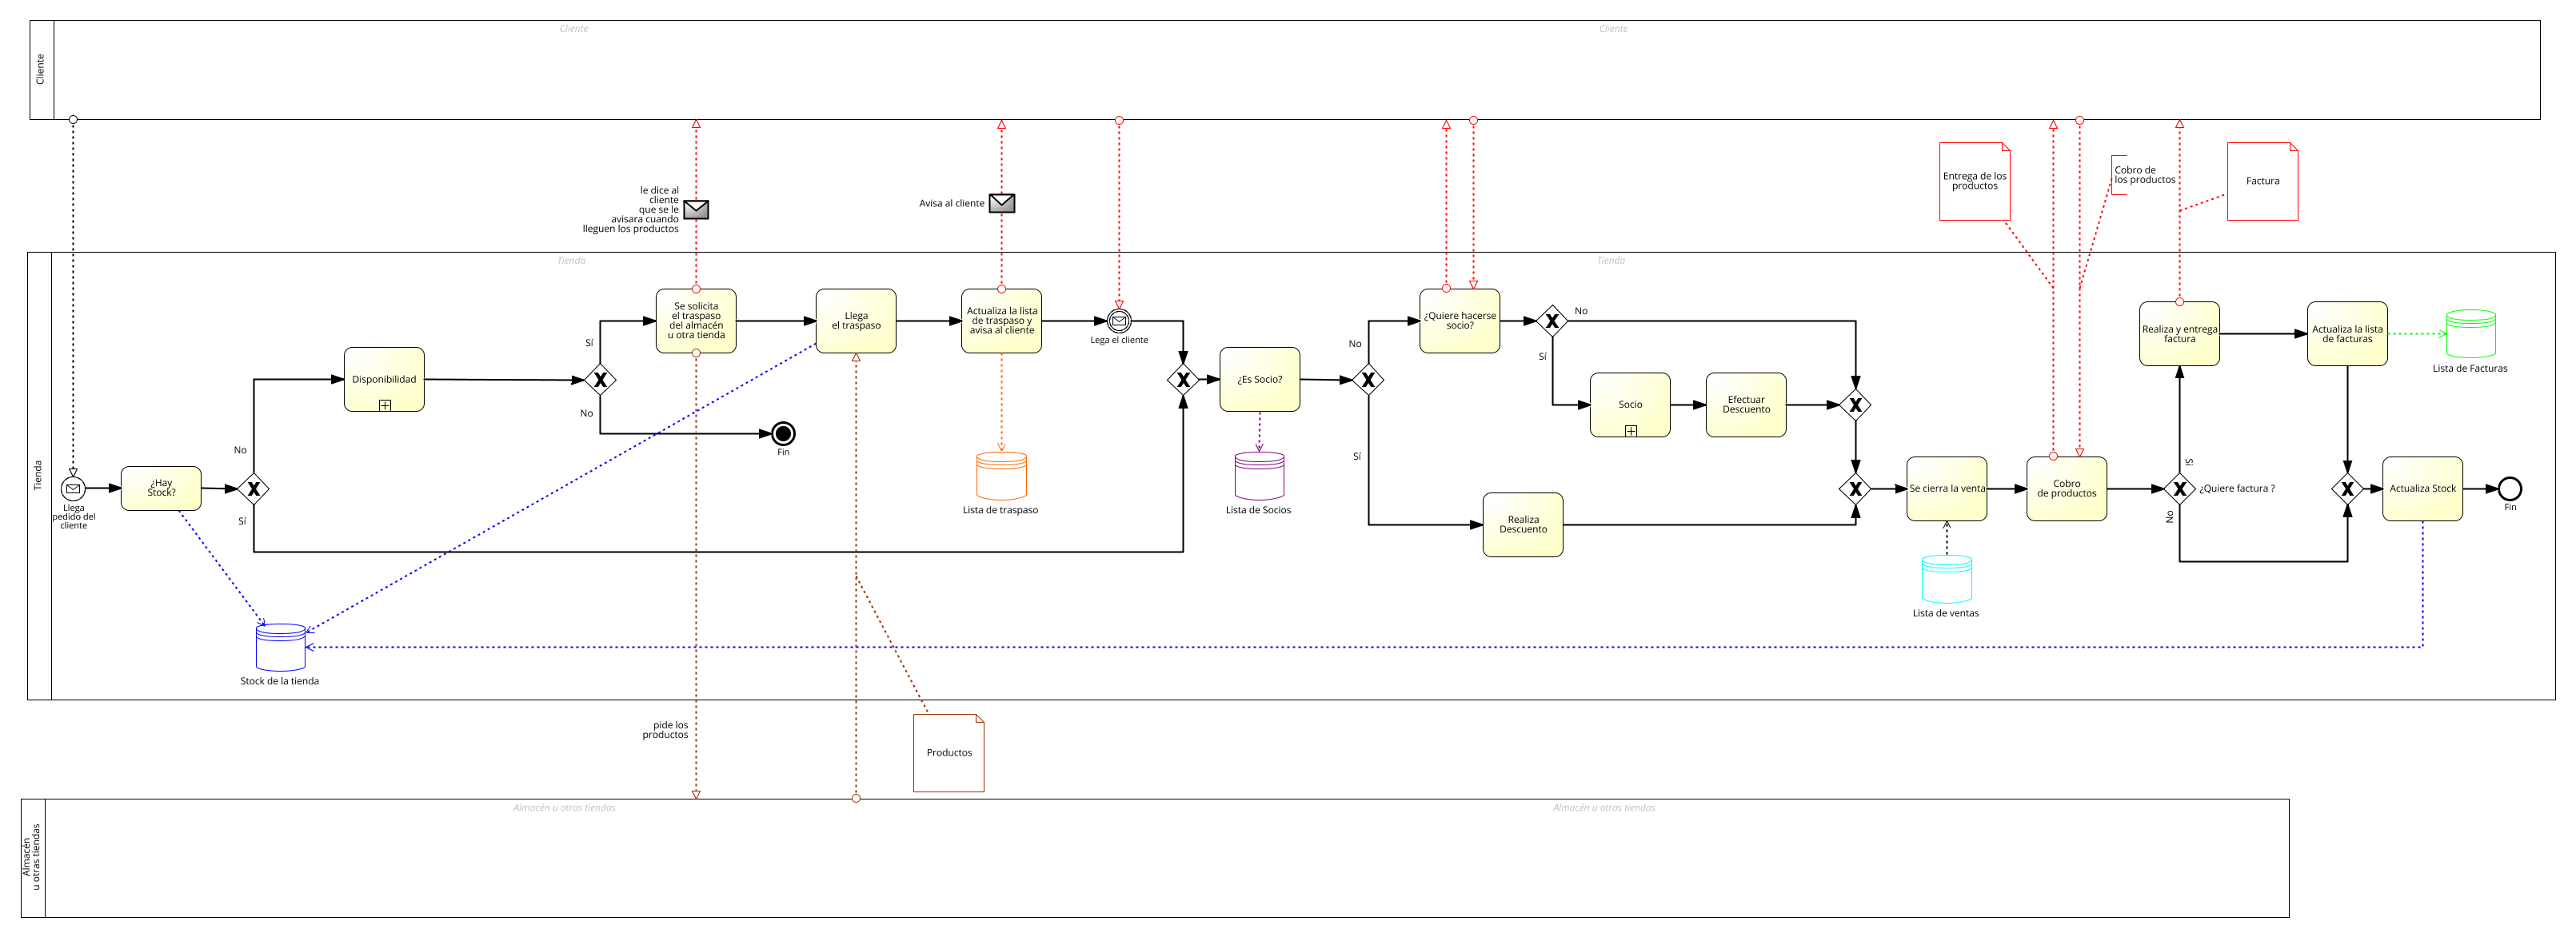
\includegraphics[width=\paperwidth, center]{images/bpmn/proceso-venta.png}
	\caption{Proceso de venta}
\end{figure}
%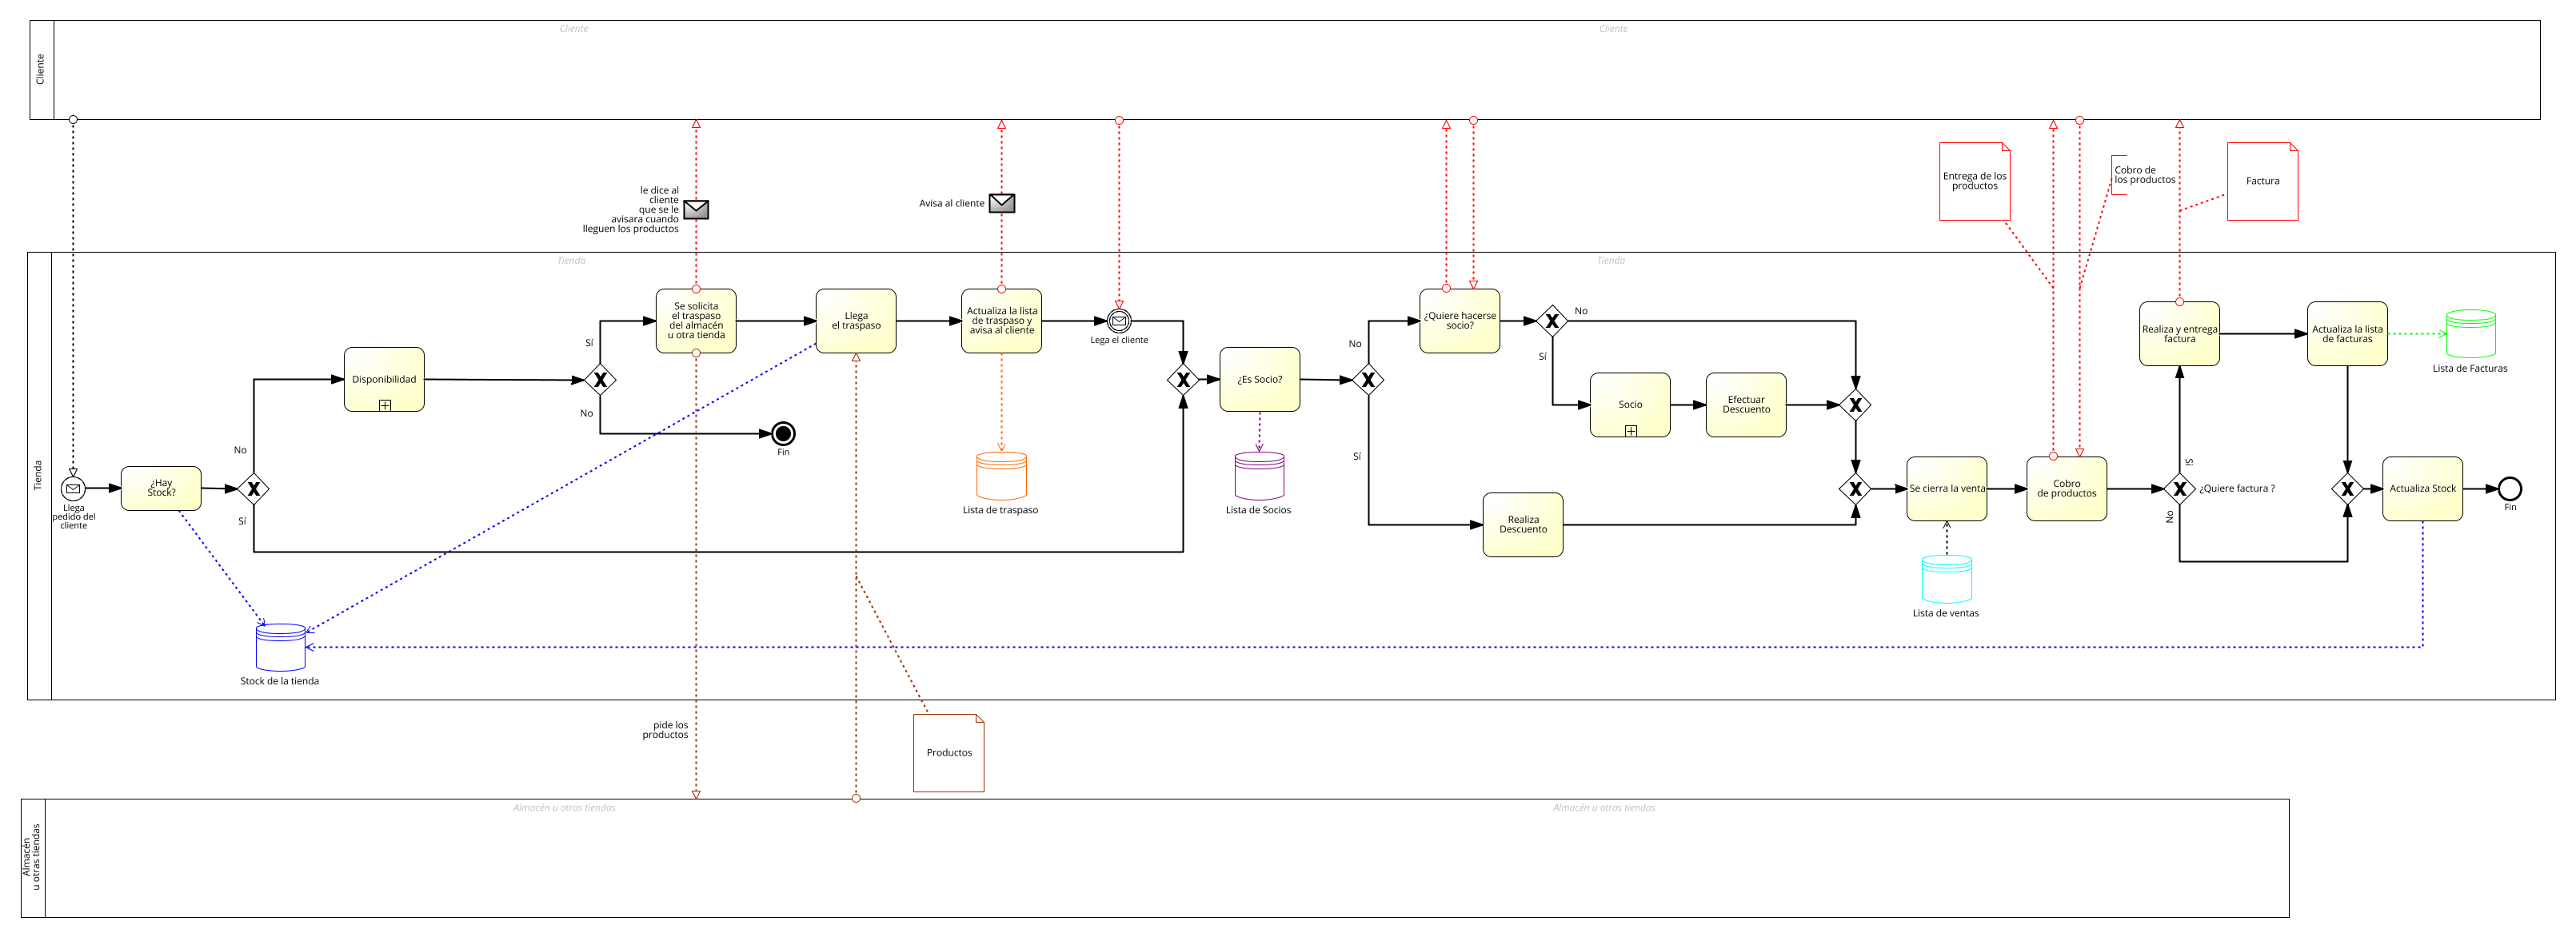
\includegraphics[width=\paperwidth, center]{images/bpmn/proceso-venta.png}
\subsection{Proceso de compra al proveedor}
\pagenumbering{gobble}
\begin{figure}[H]
	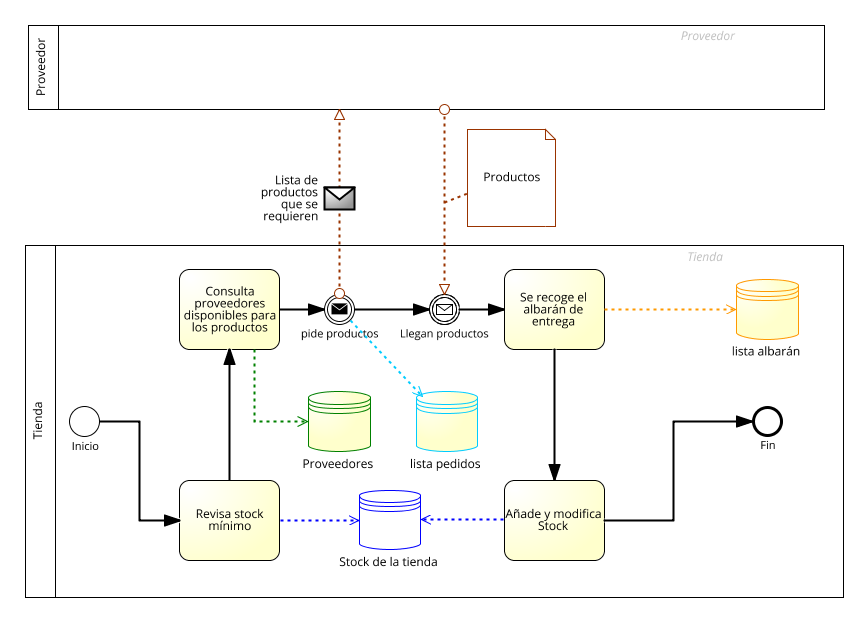
\includegraphics[width=\paperwidth, center]{images/bpmn/proceso-proveedor.png}
	\caption{Proceso de compra al proveedor}
\end{figure}
%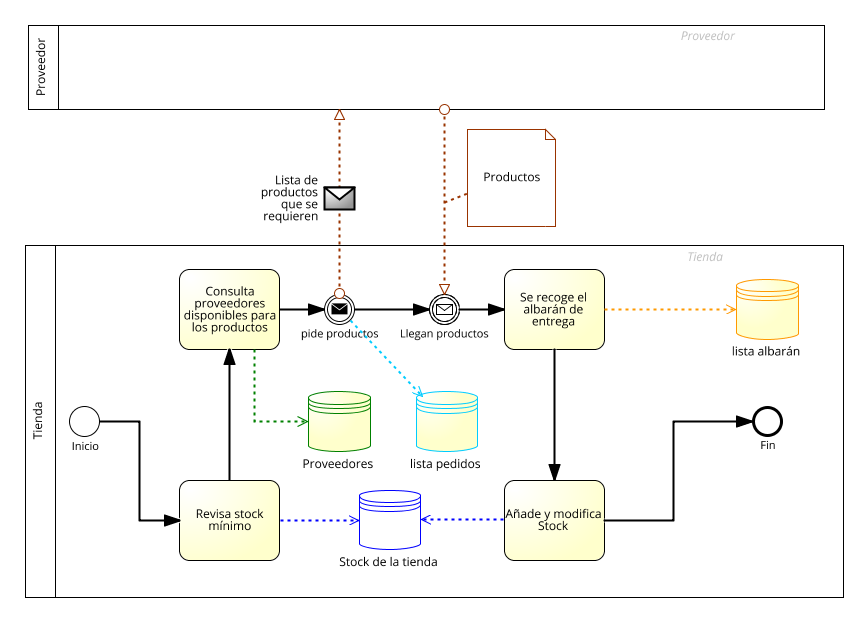
\includegraphics[width=\paperwidth, center]{images/bpmn/proceso-proveedor.png}

\subsection{Proceso de disponibilidad}
\begin{figure}[H]
	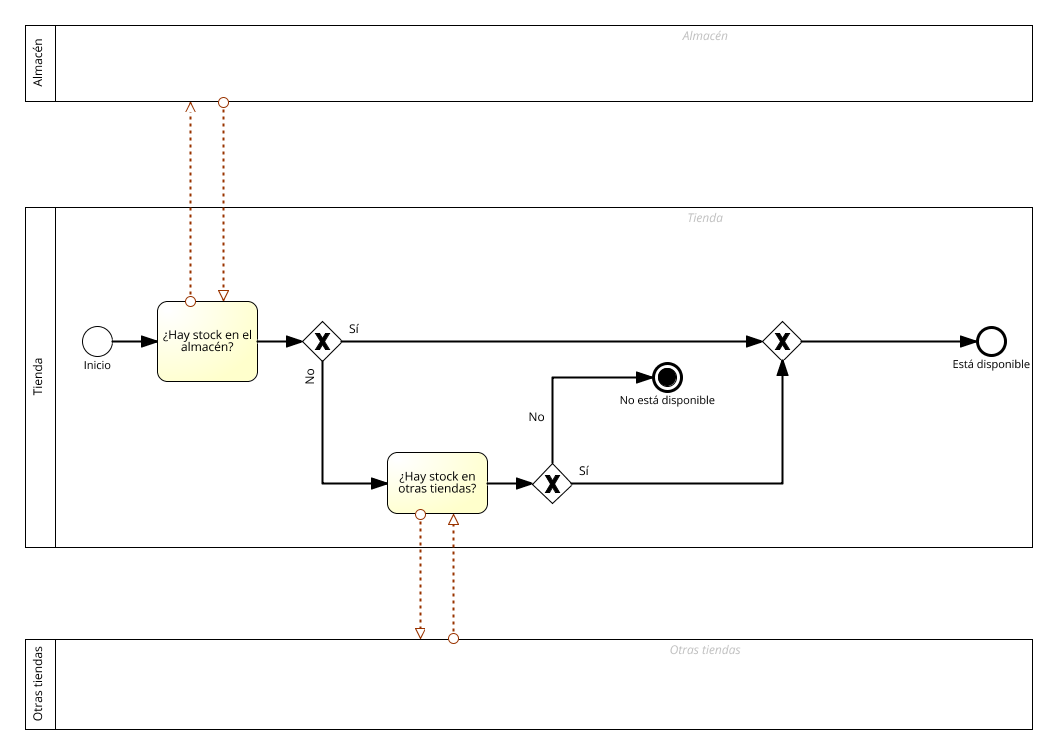
\includegraphics[width=\paperwidth, center]{images/bpmn/disponibilidad.png}
	\caption{Proceso de disponibilidad}
\end{figure}
%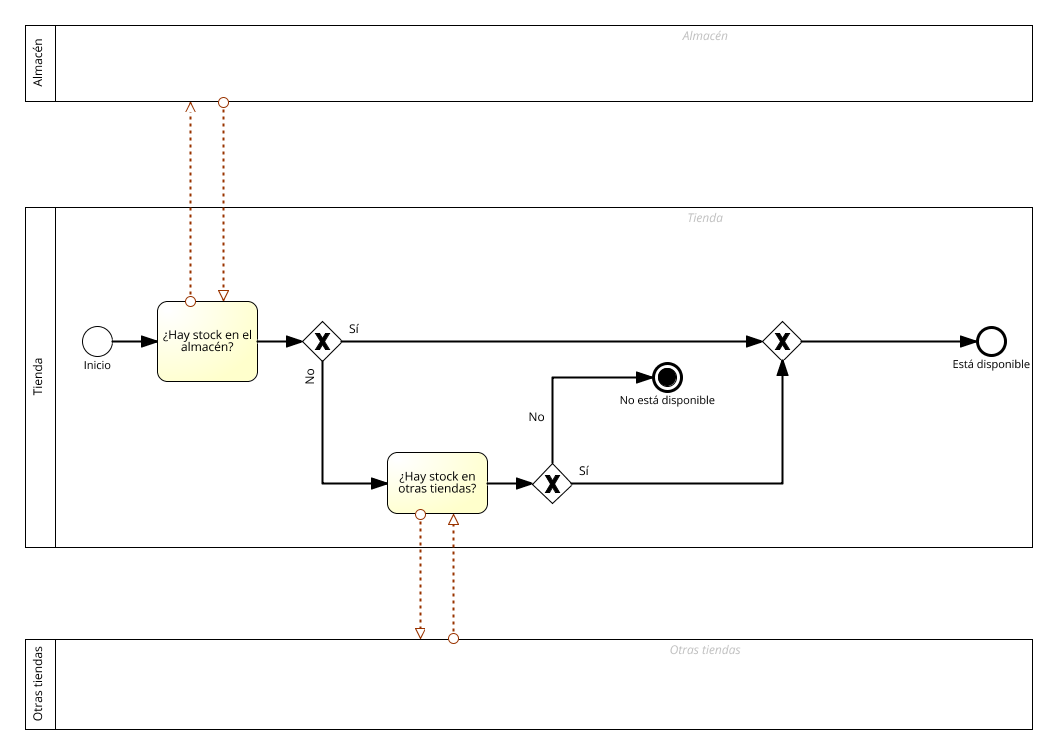
\includegraphics[width=\paperwidth, center]{images/bpmn/disponibilidad .png}

\subsection{Proceso de creación de socios}
\begin{figure}[H]
	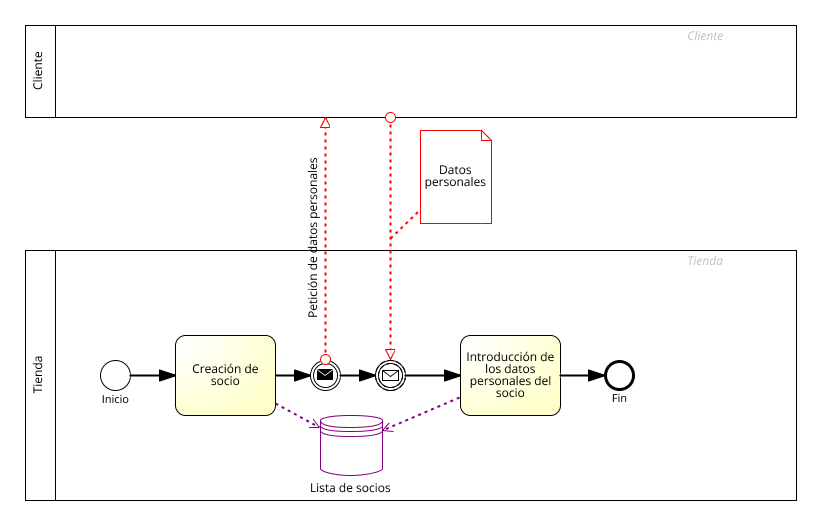
\includegraphics[width=\paperwidth, center]{images/bpmn/socios.png}
	\caption{Proceso de creación de socios}
\end{figure}
%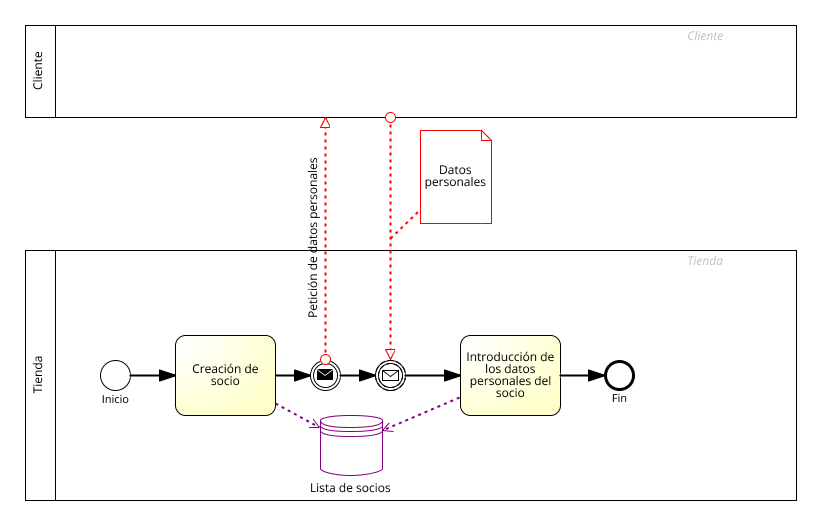
\includegraphics[width=\paperwidth, center]{images/bpmn/socios .png}
\end{landscape}

\section{Visión General del Sistema}
\subsection{Descripción}
Para solucionar los problemas planteados de clientela y gestión, el sistema estará diseñado para permitir la gestión de las ventas, los productos, los pedidos, los traspasos y los clientes de manera más eficaz.
\\\\
El objetivo principal de nuestro cliente es aumentar su clientela con la ayuda de una página web, esto lo haremos desarrollando un catálogo online de la tienda para que los clientes puedan consultar o comprar cualquier producto en cualquier momento, además de facilitar la gestión interna de la cadena.
\\\\
Con todo esto principalmente lo que se quiere es aumentar los beneficios y hacer más eficiente la gestión de la cadena.

\section{Catálogo de requisitos}

\begin{figure}[H]
	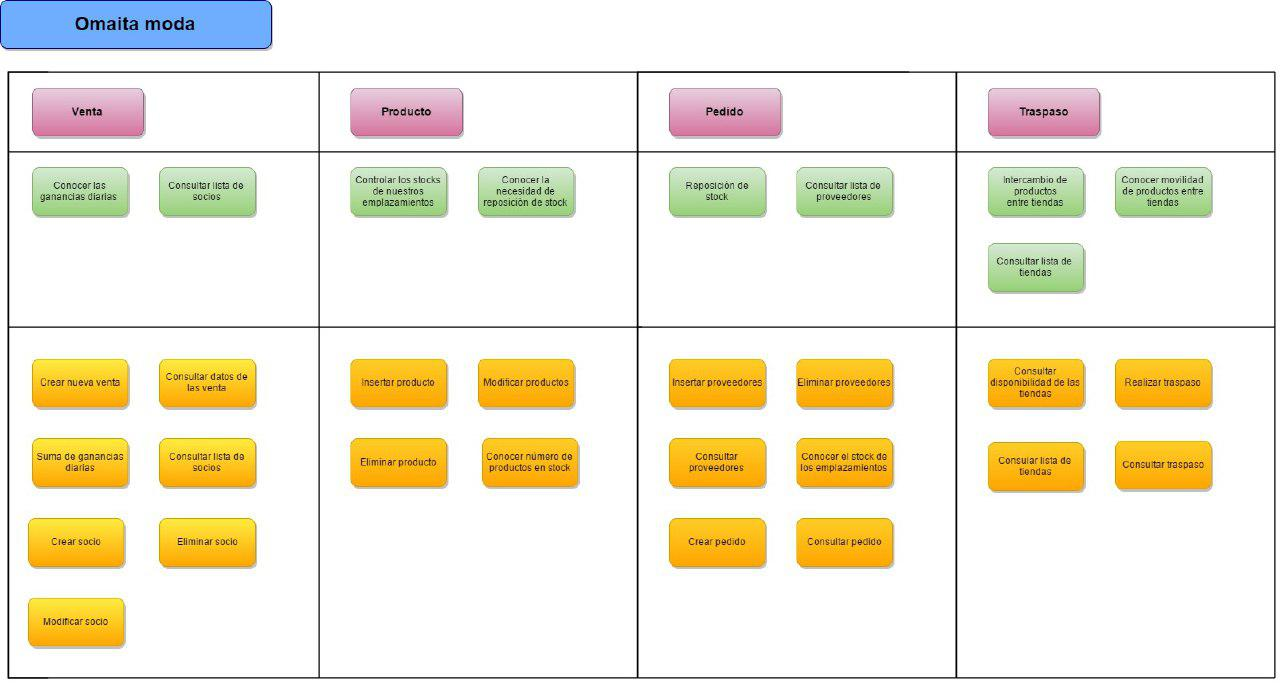
\includegraphics[width=\linewidth]{images/MapaRequisitos.jpg}
	\caption{Mapa de requisitos}
\end{figure}

\subsection{Requisitos generales}

\requit{RG-01}{Gestion ventas}{Propietario de la cadena}{poder gestionar y consultar las ventas de las tiendas}{llevar una buena gestión de ellas}
\requit{RG-02}{Gestion proveedores}{Propietario de la cadena}{poder gestionar y consultar los pedidos a proveedores}{llevar una buena gestión de ellos}
\requit{RG-03}{Traspasos}{Propietario de la cadena}{que haya un sistema de traspasos}{poder aprovechar al máximo el stock de las tiendas}
\requit{RG-04}{Catálogo}{Cliente}{poder ver una lista de los productos ofrecidos y disponibles}{realizar mis compras}

\subsection{Requisitos de información}

\requit{RI-01}{Información sobre ventas}{Propietario de la cadena}{que el sistema almacene la información correspondiente a las ventas, guardando así los siguientes datos
	\begin{itemize}
		\item Fecha en la que se llevó acabo la venta.
		\item La relación entre producto y venta que almacenará: el producto vendido, el precio y el IVA del mismo en el momento en el que se vendió.
	\end{itemize}}{conocer los datos de las ventas realizadas.}
\textbf{P-RI-01}
\begin{enumerate}
	\item Cuando se cree una nueva venta, si los datos introducidos son correctos, se almacenará en la lista de ventas.
	\item En caso de que algún dato sea incorrecto no se almacenara.
\end{enumerate}

\requit{RI-02}{Información sobre facturas}{propietario de la cadena}{que el sistema almacene la información correspondiente a las facturas, guardando así los siguientes datos:
	
	\begin{itemize}
		\item Fecha en la que se tramita la factura.
		\item Número de la factura.
		\item Un campo llamado devuelto, usado para las devoluciones, si el campo tiene el valor false, entonces podemos contabilizar esa factura sin problemas, si el campo tiene el valor true significará que el dinero fue devuelto al cliente y por la tanto no podríamos contabilizarlo.
\end{itemize}}{conocer los datos de las facturas expedidas.}
\textbf{P-RI-02}
\begin{enumerate}
	\item Cuando se cree una nueva factura, si los datos introducidos son correctos, se almacenará en la lista de factura.
	\item En caso de que algún dato sea incorrecto no se almacenara.
\end{enumerate}


\requit{RI-03}{Información sobre socios}{propietario de la cadena}{que el sistema almacene la información de los clientes que son socios, guardando los siguientes datos en él:
	\begin{itemize}
		\item Nombre.
	 	\item Apellidos.
		\item DNI.
		\item Dirección.
		\item Fecha de Nacimiento.
		\item Email.
\end{itemize}}{llevar un control de los clientes que son socios y así poderles aplicar descuentos en sus compras.}
\textbf{P-RI-03}
\begin{enumerate}
	\item Cuando se cree una nueva factura, si los datos introducidos son correctos, se almacenará en la lista de factura.
	\item En caso de que algún dato sea incorrecto (como por ejemplo un DNI duplicado) no se almacenara.
\end{enumerate}

\requit{RI-04}{Información sobre productos}{propietario de la cadena}{que los productos que venda la cadena se guarden con las siguientes características en el sistema:
	\begin{itemize}
		\item Nombre.
		\item Una breve descripción.
		\item La categoría del producto: abrigos, chaquetas, camisas, camisetas, jersey, vestidos, faldas, pantalones, calzado, accesorios y bisutería.
		\item Precio del producto.
		\item IVA actual, para controlar el IVA en todo momento
	\end{itemize}}{conocer los datos de cada producto.}
\textbf{P-RI-04}
\begin{enumerate}
	\item Cuando se inserte un nuevo producto, si los datos introducidos son correctos, se almacenará en la lista de productos.
	\item En caso de que algún dato sea incorrecto (como por ejemplo un precio negativo duplicado) no se almacenara.
\end{enumerate}


\requit{RI-05}{Stock del producto}{propietario de la cadena}{saber el stock de cada producto en cada tienda de la cadena y del almacén}{controlar el stock de la cadena}
\textbf{P-RI-05}
\begin{enumerate}
	\item Actualizar la lista de stocks cuando se cree uno nuevo o se modifique alguno ya existente.
\end{enumerate}

\requit{RI-06}{Información sobre los emplazamientos}{propietario de la cadena}{guardar la dirección de las tiendas y del almacén de la cadena, además de su teléfono de contacto}{conocer la localización de las mismas}
\textbf{P-RI-06}
\begin{enumerate}
	\item Cuando se inserte un nuevo emplazamiento, si los datos introducidos son correctos, se almacenará en la lista de emplazamientos.
	\item En caso de que algún dato sea incorrecto (como por ejemplo una dirección inexistente) no se almacenara.
\end{enumerate}

\requit{RI-07}{Información sobre los proveedores}{propietario de la cadena}{disponer de la siguiente información sobre proveedores:
	\begin{itemize}
		\item Nombre.
		\item CIF.
		\item Número de teléfono.
		\item Email.
	\end{itemize}}{saber a qué proveedores puede realizar los pedidos}
\textbf{P-RI-07}
\begin{enumerate}
	\item Cuando se inserte un nuevo proveedor, si los datos introducidos son correctos, se almacenará en la lista de proveedores.
	\item En caso de que algún dato sea incorrecto no se almacenara.
\end{enumerate}

\requit{RI-08}{Información sobre los pedidos}{propietario de la cadena}{que el sistema almacene los pedidos guardando los siguientes datos:
	\begin{itemize}
		\item Fecha en la que se realiza.
		\item Una asociación que controla la cantidad de cada producto del pedido, el precio y el IVA.
	\end{itemize}}{conocer los datos de los pedidos realizados.}
\textbf{P-RI-08}
\begin{enumerate}
	\item Cuando se inserte un nuevo pedido, si los datos introducidos son correctos, se almacenará en la lista de pedidos.
	\item En caso de que algún dato sea incorrecto no se almacenara.
\end{enumerate}

\requit{RI-09}{Información sobre traspasos}{propietario de la cadena}{que el sistema guarde los traspasos almacenando los siguientes datos:
	\begin{itemize}
		\item Fecha de traspaso.
		\item Asociación que controla la cantidad de cada producto en el traspaso.
	\end{itemize}}{conocer los datos de los traspasos realizados.}
\textbf{P-RI-09}
\begin{enumerate}
	\item Cuando se inserte un nuevo traspaso, si los datos introducidos son correctos, se almacenará en la lista de traspasos.
	\item En caso de que algún dato sea incorrecto no se almacenara.
\end{enumerate}

\requit{RI-10}{Información sobre el albarán}{propietario de la cadena}{que el sistema almacene información correspondiente a los albaranes, guardando así los siguientes datos
	\begin{itemize}
		\item Fecha de firma del albarán.
	\end{itemize}}{tener un control de los pedidos recibidos los cuales son controlados por los albaranes.}
\textbf{P-RI-10}
\begin{enumerate}
	\item Cuando se inserte un nuevo albarán, si los datos introducidos son correctos, se almacenará en la lista de albaranes.
	\item En caso de que algún dato sea incorrecto no se almacenara.
\end{enumerate}

\requit{RI-11}{Información sobre solicitud}{propietario de la cadena}{que el sistema almacene información correspondiente a las solicitudes de traspaso, guardando así los siguientes datos
	\begin{itemize}
		\item Fecha de solicitud.
		\item Asociación que controla la cantidad de cada producto en la solicitud
\end{itemize}}{conocer los datos de las solicitudes realizadas.}
\textbf{P-RI-11}
\begin{enumerate}
	\item Cuando se inserte un nuevo pedido, si los datos introducidos son correctos, se almacenará en la lista de pedidos.
	\item En caso de que algún dato sea incorrecto no se almacenara.
\end{enumerate}

\subsection{Requisitos funcionales}

\requit{RF-01}{Crear ventas}{empleado}{poder crear y consultar ventas realizadas}{poder así conocer las ganancias de la tienda}
\textbf{P-RF-01}
\begin{enumerate}
	\item Crear una nueva venta con nuevos datos y tener la posibilidad de acceder a los datos de las ventas ya realizadas.
	\item No se creará la nueva venta si algún dato introducido no es válido.
\end{enumerate}

\requit{RF-02}{Actualizar stocks tras venta}{propietario de la cadena}{que tras una factura asociada a una venta el stock se actualice}{controlar el stock de manera correcta}
\textbf{P-RF-02}
\begin{enumerate}
	\item Tras realizar una factura el stock se actualiza en función de los parámetros de las ventas asociadas a dicha factura.
\end{enumerate}

\requit{RF-03}{Crear socios}{empleado}{poder crear socios en una lista y poder consultarla}{llevar así un control sobre estos y saber si se tiene que aplicar o no el descuento.}
\textbf{P-RF-03}
\begin{enumerate}
	\item Crear un socio rellenando un formulario con los datos del cliente en cuestión.
	\item Poder acceder a la lista de los socios ya realizados.
	\item No se creará el nuevo socio si algún dato introducido no es válido.
\end{enumerate}

\requit{RF-04}{Modificar socios}{empleado}{poder modificar la dirección y el email de un socio ya creado}{tener los datos correctos del socio.}
\textbf{P-RF-04}
\begin{enumerate}
	\item Cuando se cambie algún dato de un socio, este se actualizará en la lista de socios.
	\item o se efectuará la actualización si alguno de los datos introducidos para el cambio no es valido.
\end{enumerate}

\requit{RF-05}{Eliminar socios}{empleado}{poder eliminar un socio de la base de datos}{dejar de tener almacenados los datos de un cliente que desiste de su derecho de ser socio.}
\textbf{P-RF-05}
\begin{enumerate}
	\item Cuando se elimine un socio, la lista de socios se actualizará de forma de que el socio eliminado ya no aparezca en esta.
\end{enumerate}

\requit{RF-06}{Crear, modificar y eliminar productos}{empleado}{poder insertar, modificar la descripción, el precio y el IVA de un producto, o eliminar un producto de mi base de datos}{poder así llevar una buena gestión de los productos.}
\textbf{P-RF-06}
\begin{enumerate}
	\item Insertar en la lista de productos un nuevo producto rellenando un formulario con los datos de este, y tras ello se actualizará dicha lista apareciendo en ella el nuevo producto.
	\item Cuando se cambie algún dato de un producto existente, este se actualizará en la lista de productos.
	\item Cuando se elimine un producto, la lista de productos se actualizará de forma de que el producto eliminado ya no aparezca en esta.
	\item Si algunos de los datos introducidos a la hora de insertar o actualizar un producto es incorrecto no se realizará la operación.
\end{enumerate}

\requit{RF-07}{Crear y modificar stocks}{empleado}{poder crear el stock de un producto y modificar su cantidad}{llevar un control sobre la disponibilidad de los productos según su emplazamiento.}
\textbf{P-RF-07}
\begin{enumerate}
	\item Cuando llegue un producto nuevo a la tienda se creará un stock de este con la cantidad que llegue del mismo.
	\item Cuando se realice cualquier interacción con un producto de tal forma que modifique la cantidad que existe en la tienda del mismo, se actualizara el stock.
	\item No se creará el nuevo stock si algún dato introducido no es válido, o si el producto al que se quiere realizar un stock ya posee uno en la tienda en cuestión.
\end{enumerate}

\requit{RF-08}{Crear, modificar y eliminar proveedores}{propietario de la cadena}{poder insertar, modificar el nombre, el email y el teléfono, o eliminar proveedores en mi base de datos}{conocer los proveedores disponibles y tener sus datos actualizados.}
\textbf{P-RF-08}
\begin{enumerate}
	\item Insertar en la lista de proveedores un nuevo proveedor rellenando un formulario con los datos de este, y tras ello se actualizará dicha lista apareciendo en ella el nuevo proveedor.
	\item Cuando se cambie algún dato de un proveedor existente, este se actualizará en la lista de proveedores.
	\item Cuando se elimine un proveedor, la lista de proveedores se actualizará de forma de que el proveedor eliminado ya no aparezca en esta.
	\item Si algunos de los datos introducidos a la hora de insertar o actualizar un producto es incorrecto no se realizará la operación.
\end{enumerate}

\requit{RF-09}{Crear pedidos}{empleado}{poder crear pedidos}{tener constancia de todos los pedidos realizados por cada uno de mis emplazamientos}
\textbf{P-RF-09}
\begin{enumerate}
	\item Crear un nuevo pedido con los productos que sean necesario reponer.
	\item No se podrá realizar un pedido si algún dato introducido no es válido.
\end{enumerate}

\requit{RF-10}{Actualizar stock tras pedido}{propietario de la cadena}{que tras recibir el albarán que confirma la entrega del pedido el stock se actualice}{controlar correctamente el stock.}
\textbf{P-RF-10}
\begin{enumerate}
	\item Tras recibir el pedido realizado, se actualizará la cantidad del stock de los productos del pedido.
\end{enumerate}

\requit{RF-11}{Crear solicitud de traspaso}{empleado}{poder crear una solicitud de traspaso}{así poder pedir a otra tienda productos que necesite.}
\textbf{P-RF-11}
\begin{enumerate}
	\item Poder realizar una solicitud de traspaso a otra tienda de un producto que sea necesario y esté disponible en la otra tienda.
\end{enumerate}

\requit{RF-12}{Crear traspasos}{empleado}{poder crear traspasos}{responder a la necesidad de las solicitudes de traspaso.}
\textbf{P-RF-12}
\begin{enumerate}
	\item Responder a la otra tienda siempre que sea posible cumplir con sus peticiones de solicitud de traspaso, creando en el acto un traspaso con los datos de los productos traspasados.
\end{enumerate}

\requit{RF-13}{Actualizar stock tras traspaso}{propietario de la cadena}{que cuando se realice un traspaso, se modifiquen de manera correcta los stocks de las tiendas implicadas}{así poder tener una buena gestión sobre nuestros stocks}
\textbf{P-RF-13}
\begin{enumerate}
	\item Cuando un traspaso se realiza de manera correctas ambas tiendas implicadas en el traspaso deberán actualizar la cantidad del stock de los productos implicados en el traspaso.
\end{enumerate}

\requit{RF-14}{Consultar traspasos}{propietario de la cadena}{poder consultar todos los traspasos realizados por mis emplazamientos}{conocer la movilidad de los productos entre estos.}
\textbf{P-RF-14}
\begin{enumerate}
	\item Siempre se tendrá la posibilidad de acceder a los datos de los traspasos en los que esté implicado mi tienda.
\end{enumerate}

\requit{RF-15}{Crear y eliminar emplazamientos}{propietario de la cadena}{poder añadir o eliminar emplazamientos en la base de datos}{saber que emplazamientos están en la cadena.}
\textbf{P-RF-15}
\begin{enumerate}
	\item Insertar en la lista de emplazamientos un nuevo emplazamiento rellenando un formulario con los datos de este, y tras ello se actualizará dicha lista apareciendo en ella el nuevo emplazamiento.
	\item Cuando se elimine un emplazamiento, la lista de emplazamientos se actualizará de forma de que el emplazamiento eliminado ya nTras una devolución se marcará en la factura como que se ha realizado dicha acción modificando el campo correspondiente.
	\item En el caso de que la devolución solo sea parcial y no total se creara una copia de la factura donde solo aparezcan los productos no devueltos y la antigua se marcara como devuelta.
	\item En ambos casos se actualizará el stock de los productos devueltos.
	\item Si se intenta realizar la devolución de una factura, la cual haya excedido el tiempo de devolución, no se realizará dicha devolución.o aparezca en esta.
\end{enumerate}

\requit{RF-16}{Modificar emplazamientos}{propietario de la cadena}{poder modificar la dirección y el número de teléfono de un emplazamiento}{tener los datos actualizados de mis emplazamientos.}
\textbf{P-RF-16}
\begin{enumerate}
	\item Cuando se cambie algún dato de un emplazamiento existente, este se actualizará en la lista de emplazamientos.
	\item Si al modificar algún emplazamiento se introduce algún dato no valido, no se actualizará la lista de emplazamientos.
\end{enumerate}

\requit{RF-17}{Devolución}{propietario de la cadena}{que cuando se realiza una devolución el campo devuelto de las facturas pase a ser True, y si es necesario que el empleado cree de nuevo toda la venta y la factura pero sin los productos devueltos, esta factura deberá tener el campo devuelto como False}{tener un control sobre las devoluciones.}
\textbf{P-RF-17}
\begin{enumerate}
	\item Tras una devolución se marcará en la factura como que se ha realizado dicha acción modificando el campo correspondiente.
	\item En el caso de que la devolución solo sea parcial y no total se creara una copia de la factura donde solo aparezcan los productos no devueltos y la antigua se marcara como devuelta.
	\item En ambos casos se actualizará el stock de los productos devueltos.
	\item Si se intenta realizar la devolución de una factura, la cual haya excedido el tiempo de devolución, no se realizará dicha devolución.
\end{enumerate}

\requit{RF-18}{Crear albarán}{empleado}{crear una copia del albarán de entrega que me ha dado el proveedor al traer el pedido que habíamos hecho}{tener la información de los albaranes recogida en la base de datos.}
\textbf{P-RF-18}
\begin{enumerate}
	\item Cuando llegue cualquier pedido se guardará una copia de los albaranes
\end{enumerate}


\subsection{Requisitos no funcionales}

\requit{RNF-01}{Acceso al sistema}{propietario de la cadena}{que todos mis empleados tengan acceso al sistema}{facilitar la gestión de las tiendas y el control del sistema.}

\requit{RNF-02}{Protección de datos socios}{propietario de la cadena}{que los datos de los socios permanezcan privados y seguros}{cumplir la Ley de Protección de Datos}

\requit{RNF-03}{Mantenimiento}{propietario de la cadena}{realizar el mantenimiento del sistema al menos una vez al mes}{prevenir problemas mayores en el sistema.}

\subsection{Reglas de negocio}

\requit{RN-01}{Descuento a socios}{propietario de la cadena}{aplicar un 5\% de descuento en las ventas realizadas a socios}{recompensar su fidelidad}
\textbf{P-RN-01}
\begin{enumerate}
	\item Cuando se realice una venta, si esta está asociada a un socio , se aplicara el descuento en la factura.
\end{enumerate}

\requit{RN-02}{Tamaño mínimo de pedidos}{propietario de la cadena quiero}{que los pedidos sean como mínimo de 20 unidades por producto}{abaratar gastos de transporte.}
\textbf{P-RN-02}
\begin{enumerate}
	\item Cuando se realice un pedido, si la cantidad de algún producto no supera el mínimo no se realizará dicho pedido, en caso contrario se realizara sin ningún problema.
\end{enumerate}

\requit{RN-03}{Evitar traspaso si se provoca stock mínimo}{propietario de la cadena}{que las tiendas no puedan ofrecer el traspaso de un producto, si debido al traspaso el producto llega a su stock mínimo}{evitar que éstas se queden desabastecidas}
\textbf{P-RN-03}
\begin{enumerate}
	\item No se podrá responder a una solicitud de traspaso si en caso de realizar el traspaso el producto solicitado se nos quedaría en stock mínimo
\end{enumerate}

\requit{RN-04}{Política de devoluciones}{propietario de la cadena}{que solo se acepten devoluciones, con un plazo máximo de 30 días después de la compra}{dificultar la devolución de productos usados}
\textbf{P-RN-04}
\begin{enumerate}
	\item Si se intenta realizar una devolución dentro del plazo de devolución establecido por la tienda (en nuestro caso 30 días a partir del día de la compra) se permite realizar dicha devolución ya sea total o parcial.
	\item En caso contrario no se podrá realizar la devolución.
\end{enumerate}

\requit{RN-05}{Aviso stock mínimo}{trabajador de una tienda}{obtener un aviso cuando el stock de un producto llegue al stock mínimo}{evitar el desabastecimiento de un producto}
\textbf{P-RN-05}
\begin{enumerate}
	\item Cuando un producto este bajo el stock mínimo saltara un mensaje de aviso para tener en cuenta su futura reposición 
\end{enumerate}

\section{Modelo Conceptual}
\subsection{Diagramas de clases UML}

\begin{figure}[H]
	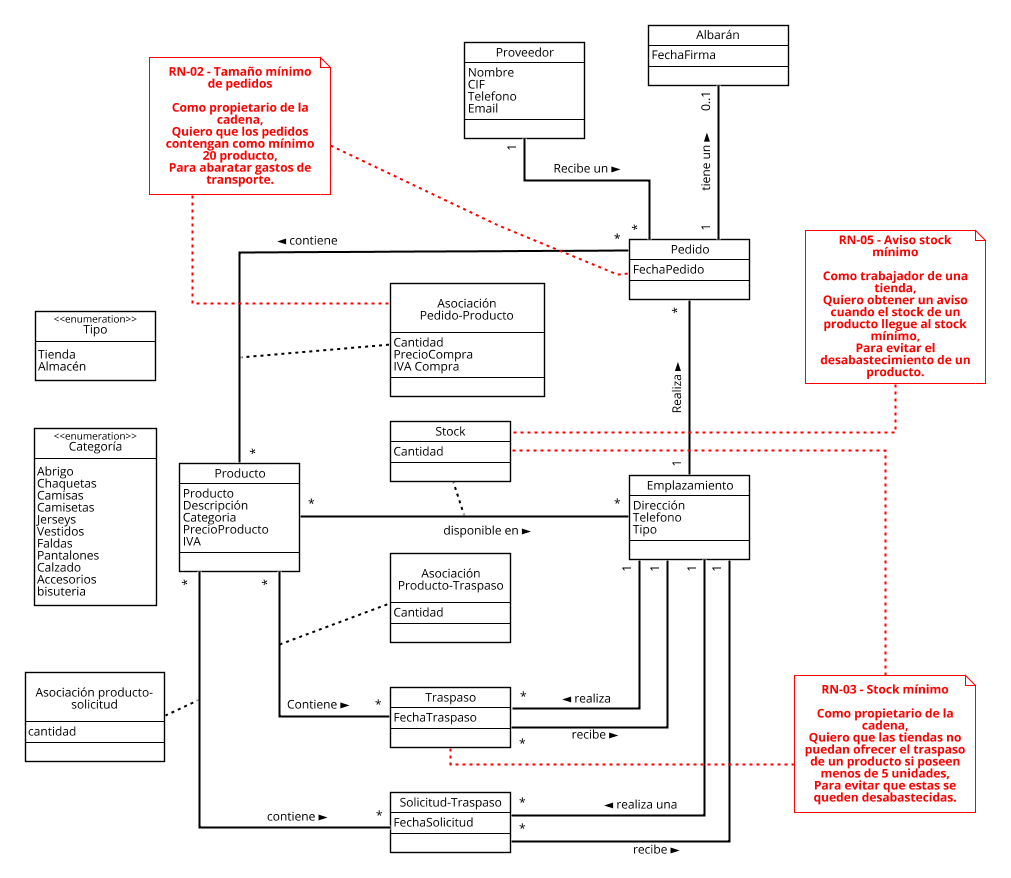
\includegraphics[width=\linewidth]{images/UML-traspaso-pedido.png}
	\caption{UML Traspaso / Pedido}
\end{figure}

\begin{figure}[H]
	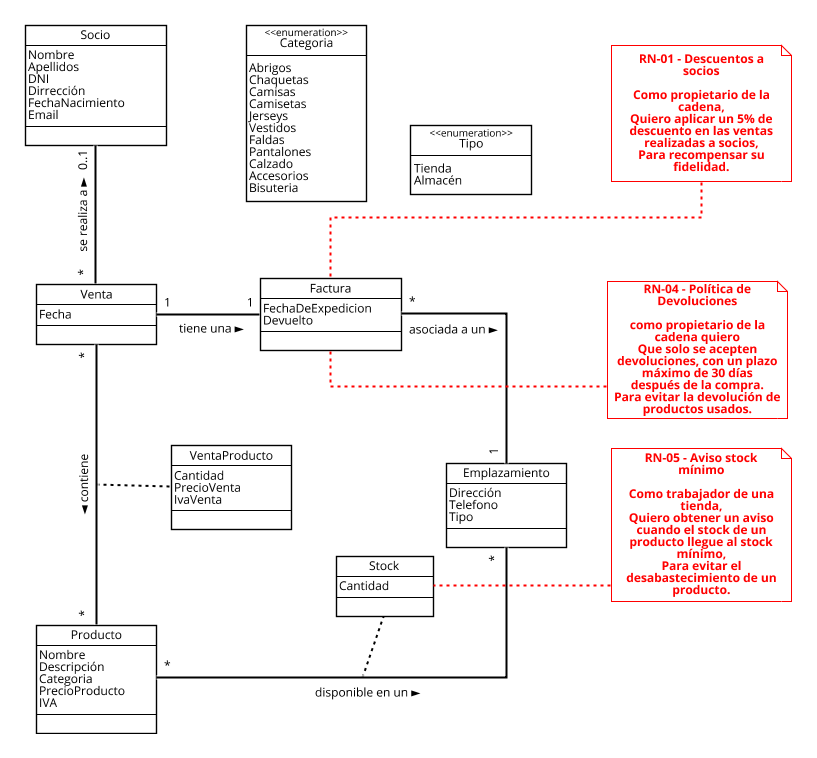
\includegraphics[width=\linewidth]{images/UML-venta.png}
	\caption{UML Venta}
\end{figure}

\subsection{Escenarios de prueba}

\begin{figure}[H]
	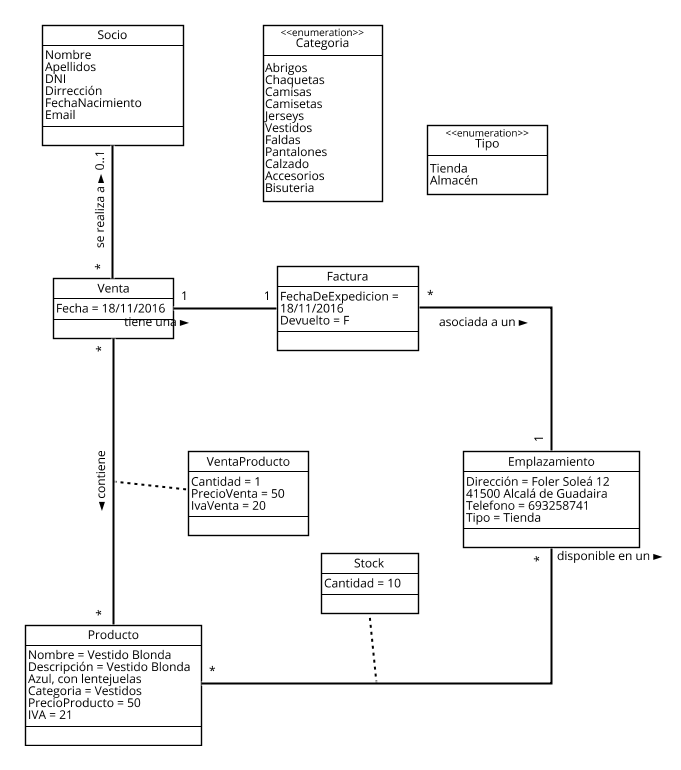
\includegraphics[width=\linewidth]{images/pruebas/venta-no-socio.png}
	\caption{UML Venta NO Socio}
\end{figure}

\begin{figure}[H]
	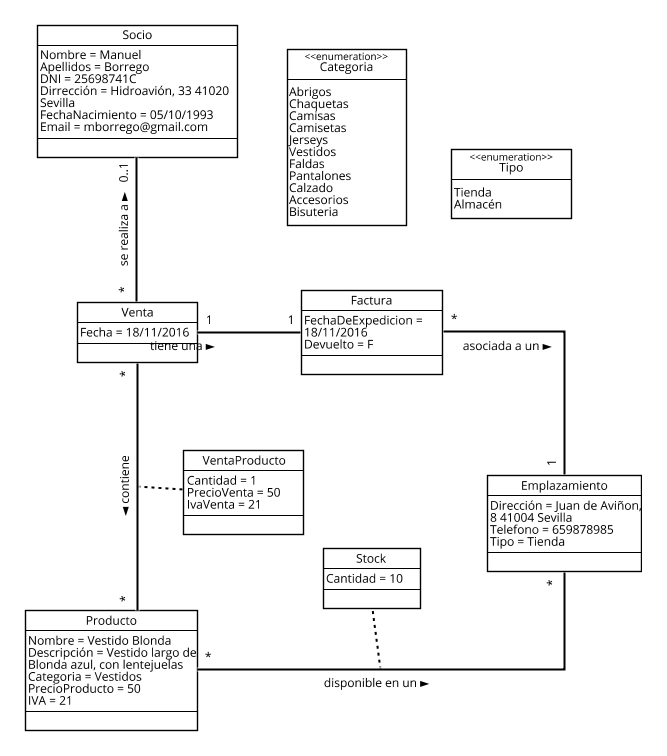
\includegraphics[width=\linewidth]{images/pruebas/venta-socio.png}
	\caption{UML Venta Socio}
\end{figure}

\begin{figure}[H]
	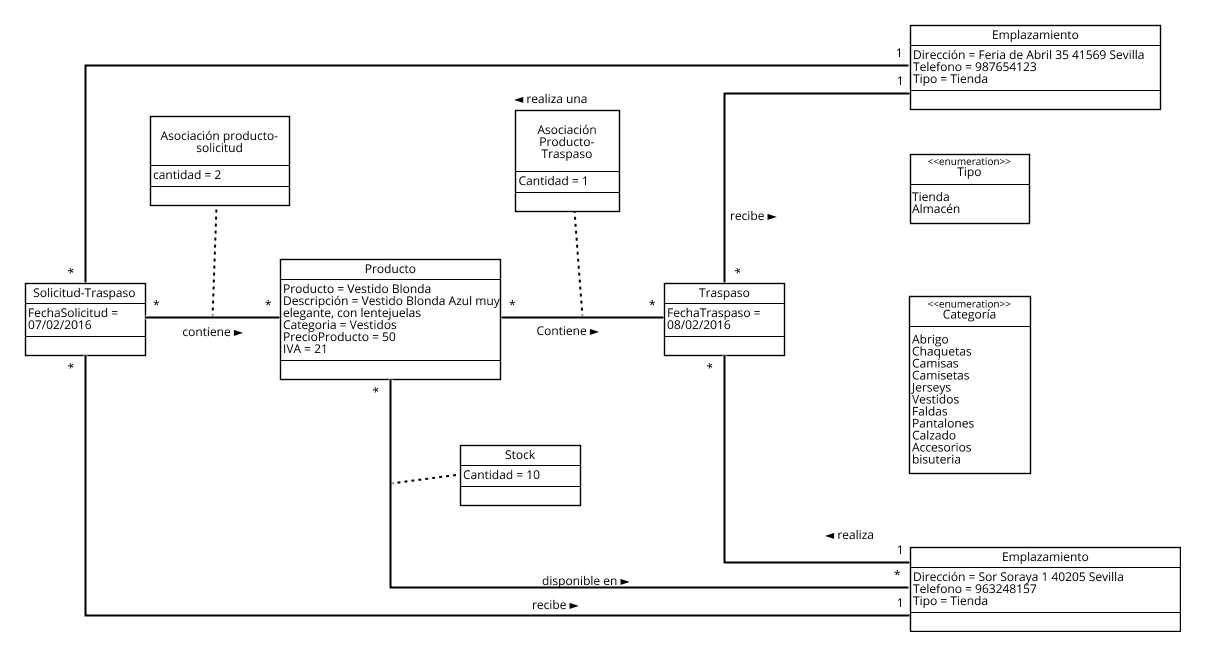
\includegraphics[width=\linewidth]{images/pruebas/traspaso-tienda-tienda.png}
	\caption{UML Traspaso Tienda - Tienda}
\end{figure}

\begin{figure}[H]
	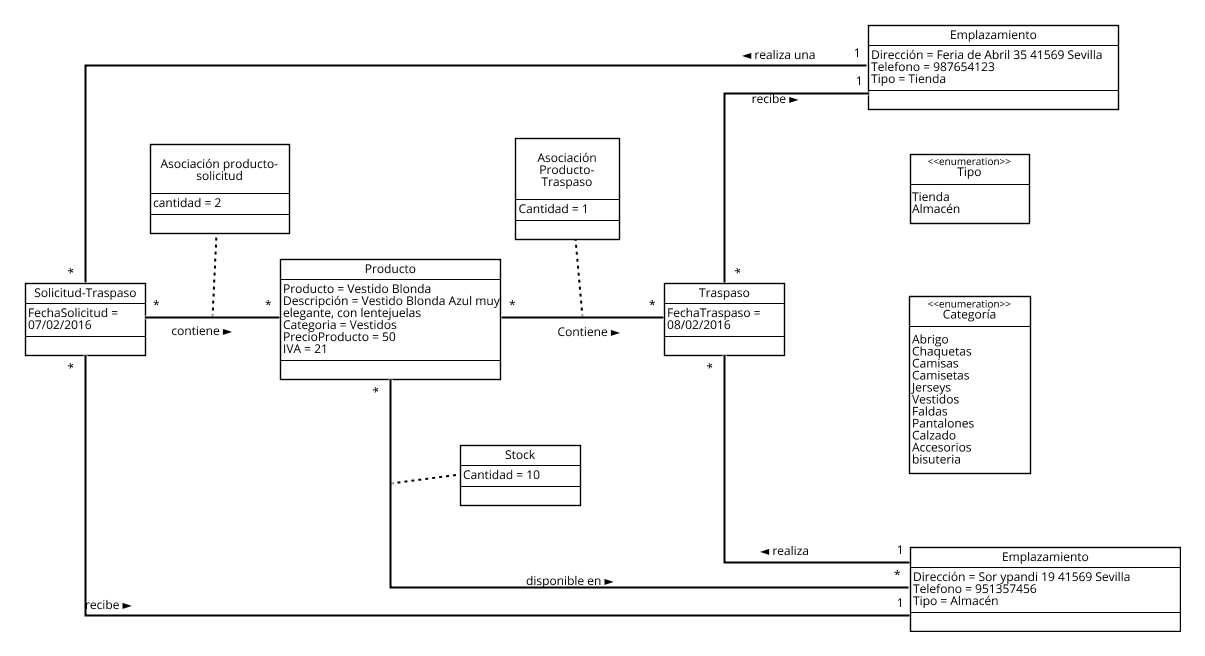
\includegraphics[width=\linewidth]{images/pruebas/traspaso-tienda-almacen.png}
	\caption{UML Traspaso Tienda - Almacén}
\end{figure}

\begin{figure}[H]
	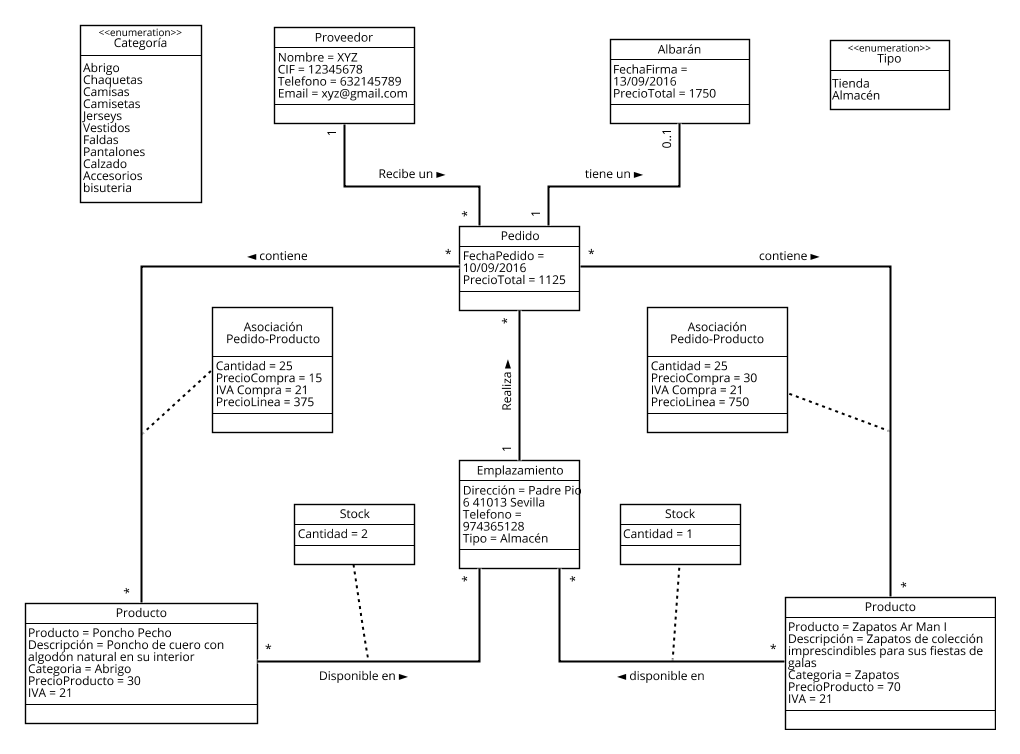
\includegraphics[width=\linewidth]{images/pruebas/pedido-tienda-proveedor.png}
	\caption{UML Pedido Tienda - Proveedor}
\end{figure}

\begin{figure}[H]
	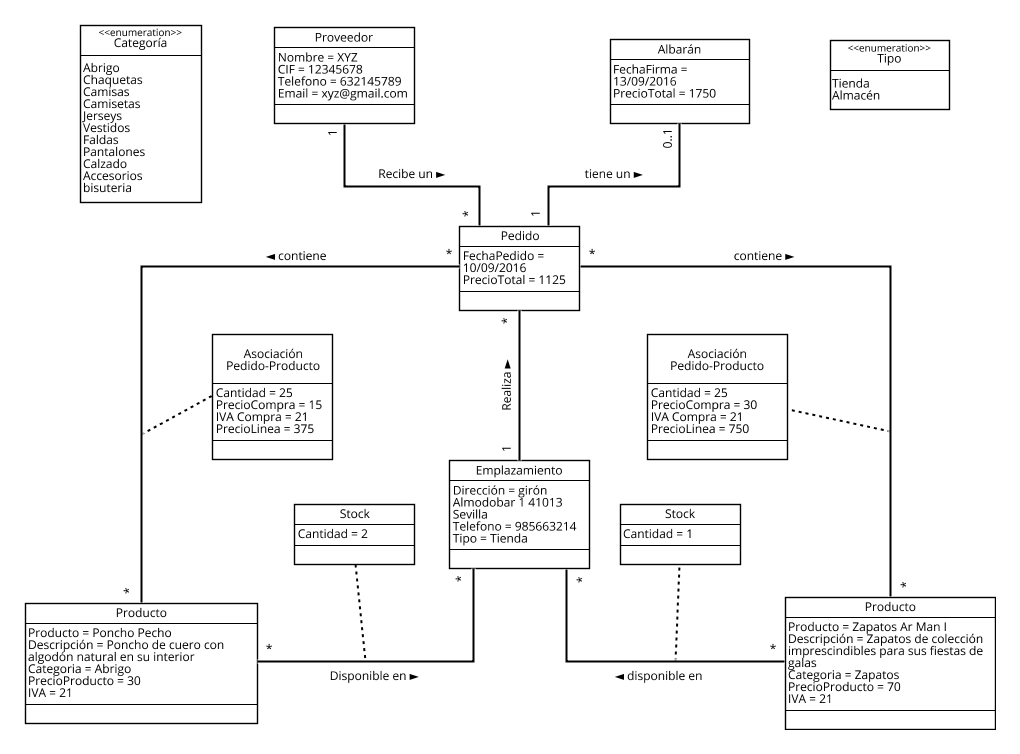
\includegraphics[width=\linewidth]{images/pruebas/pedido-almacen-proveedor.png}
	\caption{UML Pedido Almacén - Proveedor}
\end{figure}

\section{Matrices de trazabilidad}

\subsection{Pruebas de aceptación frente a requisitos}

\begin{table}[H]
	\centering
	\caption{\textbf{Requisitos funcionales}}
	\label{Requisitos funcionales}
	\resizebox{\textwidth}{!}{\begin{tabular}{|c|c|c|c|c|c|c|c|c|c|c|c|c|c|c|c|c|c|c|}
			\hline
			\textbf{P-RF-01} & X             &               &               &               &               &               &               &               &               &               &               &               &               &               &               &               &               &               \\ \hline
			\textbf{P-RF-02} &               & X             &               &               &               &               &               &               &               &               &               &               &               &               &               &               &               &               \\ \hline
			\textbf{P-RF-03} &               &               & X             &               &               &               &               &               &               &               &               &               &               &               &               &               &               &               \\ \hline
			\textbf{P-RF-04} &               &               &               & X             &               &               &               &               &               &               &               &               &               &               &               &               &               &               \\ \hline
			\textbf{P-RF-05} &               &               &               &               & X             &               &               &               &               &               &               &               &               &               &               &               &               &               \\ \hline
			\textbf{P-RF-06} &               &               &               &               &               & X             &               &               &               &               &               &               &               &               &               &               &               &               \\ \hline
			\textbf{P-RF-07} &               &               &               &               &               &               & X             &               &               &               &               &               &               &               &               &               &               &               \\ \hline
			\textbf{P-RF-08} &               &               &               &               &               &               &               & X             &               &               &               &               &               &               &               &               &               &               \\ \hline
			\textbf{P-RF-09} &               &               &               &               &               &               &               &               & X             &               &               &               &               &               &               &               &               &               \\ \hline
			\textbf{P-RF-10} &               &               &               &               &               &               &               &               &               & X             &               &               &               &               &               &               &               &               \\ \hline
			\textbf{P-RF-11} &               &               &               &               &               &               &               &               &               &               & X             &               &               &               &               &               &               &               \\ \hline
			\textbf{P-RF-12} &               &               &               &               &               &               &               &               &               &               &               & X             &               &               &               &               &               &               \\ \hline
			\textbf{P-RF-13} &               &               &               &               &               &               &               &               &               &               &               &               & X             &               &               &               &               &               \\ \hline
			\textbf{P-RF-14} &               &               &               &               &               &               &               &               &               &               &               &               &               & X             &               &               &               &               \\ \hline
			\textbf{P-RF-15} &               &               &               &               &               &               &               &               &               &               &               &               &               &               & X             &               &               &               \\ \hline
			\textbf{P-RF-16} &               &               &               &               &               &               &               &               &               &               &               &               &               &               &               & X             &               &               \\ \hline
			\textbf{P-RF-17} &               &               &               &               &               &               &               &               &               &               &               &               &               &               &               &               & X             &               \\ \hline
			\textbf{P-RF-18} &               &               &               &               &               &               &               &               &               &               &               &               &               &               &               &               &               & X             \\ \hline
			\textbf{}        & \textbf{01} & \textbf{02} & \textbf{03} & \textbf{04} & \textbf{05} & \textbf{06} & \textbf{07} & \textbf{08} & \textbf{09} & \textbf{10} & \textbf{11} & \textbf{12} & \textbf{13} & \textbf{14} & \textbf{15} & \textbf{16} & \textbf{17} & \textbf{18} \\ \hline
	\end{tabular}}
\end{table}

\begin{table}[H]
	\centering
	\caption{\textbf{Requisitos de información}}
	\label{Requisitos de informacion}
	\resizebox{\textwidth}{!}{\begin{tabular}{|c|c|c|c|c|c|c|c|c|c|c|c|}
			\hline
			\textbf{P-RI-01} & X           &             &             &             &             &             &             &             &             &             &             \\ \hline
			\textbf{P-RI-02} &             & X           &             &             &             &             &             &             &             &             &             \\ \hline
			\textbf{P-RI-03} &             &             & X           &             &             &             &             &             &             &             &             \\ \hline
			\textbf{P-RI-04} &             &             &             & X           &             &             &             &             &             &             &             \\ \hline
			\textbf{P-RI-05} &             &             &             &             & X           &             &             &             &             &             &             \\ \hline
			\textbf{P-RI-06} &             &             &             &             &             &    X        &             &             &             &             &             \\ \hline
			\textbf{P-RI-07} &             &             &             &             &             &             &  X          &             &             &             &             \\ \hline
			\textbf{P-RI-08} &             &             &             &             &             &             &             & X           &             &             &             \\ \hline
			\textbf{P-RI-09} &             &             &             &             &             &             &             &             &  X          &             &             \\ \hline
			\textbf{P-RI-10} &             &             &             &             &             &             &             &             &             & X           &             \\ \hline
			\textbf{P-RI-11} &             &             &             &             &             &             &             &             &             &             & X           \\ \hline
			\textbf{}      & \textbf{01} & \textbf{02} & \textbf{03} & \textbf{04} & \textbf{05} & \textbf{06} & \textbf{07} & \textbf{08} & \textbf{09} & \textbf{10} & \textbf{11} \\ \hline
	\end{tabular}}
\end{table}

\begin{table}[H]
	\centering
	\caption{\textbf{Reglas de negocio}}
	\label{Reglas de negocio}
	\begin{tabular}{|c|c|c|c|c|c|}
		\hline
		\textbf{P-RN-01} & X           &             &             &             &             \\ \hline
		\textbf{P-RN-02} &             &   X         &             &             &             \\ \hline
		\textbf{P-RN-03} &             &             &     X       &             &             \\ \hline
		\textbf{P-RN-04} &             &             &             & X           &             \\ \hline
		\textbf{P-RN-05} &             &             &             &             & X           \\ \hline
		\textbf{}      & \textbf{01} & \textbf{02} & \textbf{03} & \textbf{04} & \textbf{05} \\ \hline
	\end{tabular}
\end{table}

\subsection{Pruebas de aceptación frente a escenarios de prueba}

\begin{table}[H]
	\centering
	\caption{\textbf{Escenarios}}
	\label{Escenarios}
	\resizebox{\textwidth}{!}{\begin{tabular}{|c|c|c|c|c|c|c|c|c|c|c|c|}
		\hline
		\textbf{Escenario 01} & X                & X                & X                & X                & X                & X                &                  &                  &                  &                  &                  \\ \hline
		\textbf{Escenario 02} & X                & X                & X                & X                & X                & X                &                  &                  &                  &                  &                  \\ \hline
		\textbf{Escenario 03} &                  &                  &                  & X                & X                & X                &                  &                  & X                &                  &                  \\ \hline
		\textbf{Escenario 04} &                  &                  &                  & X                & X                & X                &                  &                  & X                &                  &                  \\ \hline
		\textbf{Escenario 05} &                  &                  &                  & X                & X                & X                & X                & X                &                  & X                & X                \\ \hline
		\textbf{Escenario 06} &                  &                  &                  & X                & X                & X                & X                & X                &                  & X                & X                \\ \hline
		\textbf{}             & \textbf{P-RI-01} & \textbf{P-RI-02} & \textbf{P-RI-03} & \textbf{P-RI-04} & \textbf{P-RI-05} & \textbf{P-RI-06} & \textbf{P-RI-07} & \textbf{P-RI-08} & \textbf{P-RI-09} & \textbf{P-RI-10} & \textbf{P-RI-11} \\ \hline
	\end{tabular}}
\end{table}

\begin{table}[H]
	\centering
	\caption{\textbf{Escenarios}}
	\label{Escenarios}
	\resizebox{\textwidth}{!}{\begin{tabular}{|c|c|c|c|c|c|c|c|c|c|c|c|c|c|c|c|c|c|c|}
			\hline
			\textbf{Escenario 01} & X                & X                &                  &                  &                  & X                &                  &                  &                  &                  &                  &                  &                  &                  & X                & X                & X                &                  \\ \hline
			\textbf{Escenario 02} & X                & X                & X                & X                & X                & X                &                  &                  &                  &                  &                  &                  &                  &                  & X                & X                & X                &                  \\ \hline
			\textbf{Escenario 03} &                  &                  &                  &                  &                  & X                &                  &                  &                  &                  & X                & X                & X                & X                & X                & X                &                  &                  \\ \hline
			\textbf{Escenario 04} &                  &                  &                  &                  &                  & X                & X                &                  &                  &                  & X                & X                & X                & X                & X                & X                &                  &                  \\ \hline
			\textbf{Escenario 05} &                  &                  &                  &                  &                  & X                & X                & X                & X                & X                &                  &                  &                  &                  & X                & X                &                  & X                \\ \hline
			\textbf{Escenario 06} &                  &                  &                  &                  &                  & X                & X                & X                & X                & X                &                  &                  &                  &                  & X                & X                &                  & X                \\ \hline
			\textbf{}             & \textbf{P-RF-01} & \textbf{P-RF-02} & \textbf{P-RF-03} & \textbf{P-RF-04} & \textbf{P-RF-05} & \textbf{P-RF-06} & \textbf{P-RF-07} & \textbf{P-RF-08} & \textbf{P-RF-09} & \textbf{P-RF-10} & \textbf{P-RF-11} & \textbf{P-RF-12} & \textbf{P-RF-13} & \textbf{P-RF-14} & \textbf{P-RF-15} & \textbf{P-RF-16} & \textbf{P-RF-17} & \textbf{P-RF-18} \\ \hline
	\end{tabular}}
\end{table}

\begin{table}[H]
	\centering
	\caption{\textbf{Escenarios}}
	\label{Escenarios}
	\resizebox{\textwidth}{!}{\begin{tabular}{|c|c|c|c|c|c|}
			\hline
			\textbf{Escenario 01} & X                &                  &                  & X                & X                \\ \hline
			\textbf{Escenario 02} & X                &                  &                  & X                & X                \\ \hline
			\textbf{Escenario 03} &                  &                  & X                &                  & X                \\ \hline
			\textbf{Escenario 04} &                  &                  & X                &                  & X                \\ \hline
			\textbf{Escenario 05} &                  & X                &                  &                  & X                \\ \hline
			\textbf{Escenario 06} &                  & X                &                  &                  & X                \\ \hline
			\textbf{}             & \textbf{P-RN-01} & \textbf{P-RN-02} & \textbf{P-RN-03} & \textbf{P-RN-04} & \textbf{P-RN-05} \\ \hline
	\end{tabular}}
\end{table}

\subsection{Tipos de UML frente a Requisitos}

\begin{table}[H]
	\centering
	\caption{\textbf{Requisitos de informacion}}
	\resizebox{\textwidth}{!}{\begin{tabular}{|c|l|l|l|l|l|l|l|l|l|l|l|}
		\hline
		\textbf{Venta}             & x                                & x                                & x                                & x                                & x                                & x                                &                                  &                                  &                                  &                                  &                                  \\ \hline
		\textbf{Traspaso - Pedido} &                                  &                                  &                                  & x                                & x                                & x                                & x                                & x                                & x                                & x                                & x                                \\ \hline
		\textbf{}                  & \multicolumn{1}{c|}{\textbf{01}} & \multicolumn{1}{c|}{\textbf{02}} & \multicolumn{1}{c|}{\textbf{03}} & \multicolumn{1}{c|}{\textbf{04}} & \multicolumn{1}{c|}{\textbf{05}} & \multicolumn{1}{c|}{\textbf{06}} & \multicolumn{1}{c|}{\textbf{07}} & \multicolumn{1}{c|}{\textbf{08}} & \multicolumn{1}{c|}{\textbf{09}} & \multicolumn{1}{c|}{\textbf{10}} & \multicolumn{1}{c|}{\textbf{11}} \\ \hline
	\end{tabular}}
\end{table}

\begin{table}[H]
	\centering
	\caption{\textbf{Reglas de negocio}}
	\begin{tabular}{|c|c|c|c|c|c|}
		\hline
		\textbf{Venta}             & x           &             &             & x           & x           \\ \hline
		\textbf{Traspaso - Pedido} &             & x           & x           &             & x           \\ \hline
		\textbf{}                  & \textbf{01} & \textbf{02} & \textbf{03} & \textbf{04} & \textbf{05} \\ \hline
	\end{tabular}
\end{table}

\begin{table}[H]
	\centering
	\caption{\textbf{Requisitos Funcionales}}
	\resizebox{\textwidth}{!}{\begin{tabular}{|c|c|c|c|c|c|c|c|c|c|c|c|c|c|c|c|c|c|c|}
		\hline
		\textbf{Venta}            & X           & X           & X           & X           & X           & X           & X           &             &             &             &             &             &             &             & X           & X           & X           &             \\ \hline
		\textbf{Traspaso - Venta} &             &             &             &             &             & X           & X           & X           & X           & X           & X           & X           & X           & X           & X           & X           &             & X           \\ \hline
		\textbf{}                 & \textbf{01} & \textbf{02} & \textbf{03} & \textbf{04} & \textbf{05} & \textbf{06} & \textbf{07} & \textbf{08} & \textbf{09} & \textbf{10} & \textbf{11} & \textbf{12} & \textbf{13} & \textbf{14} & \textbf{15} & \textbf{16} & \textbf{17} & \textbf{18} \\ \hline
	\end{tabular}}
\end{table}

\section{Modelos relacionales}
Para poder pasar de UML(MC) a 3FN(MR), tenemos que ser capaces de normalizar tanto en 2FN como en 1FN,
esto lo hemos comprobado de la siguiente manera:
En cada tupla de la 3FN se le asigna a cada atributo un solo valor del dominio sobre el que está definido, es decir, no existen atributos con
varios valores. Esto prueba que está en 1FN.
Tras asegurar la 1FN, pasamos a la comprobación de la 2FN, para validar esta normalización tenemos que tener en cuenta que los atributos que no
sean Primary Key o Foreign Key (atributos no primos) deben de ser dependientes de estas claves, esto lo cumplimos gracias a las foreign keys y
primary keys creadas para las asociaciones, esta relación está explicada más adelante.
Finalmente llegamos a la comprobación de la 3FN, para esta comprobación tenemos que tener en cuenta que la relación tiene que estar en 2FN y que
la relación de tablas simplemente se haga mediante las primary y las foreign key, todo lo que no sea claves candidatas no puede estar en
varias entidades asociadas a la vez.

\subsection{3FN Venta}

 \begin{itemize}
 	\item[Socio] Los atributos son directos en la 3FN, añadiendo que DNI será una primray key. Tiene una relación 0..1 - n con Venta, venta mantiene todos sus atributos de manera directa en la 3FN, añadiendo un ID\_VENTA como
primary key y debido a la relación con socio una foreign key llamada DNI.
 	\item[Venta] Tiene una relación n - m con Producto, se crea una tabla intermedia debido a esta relación que es la tabla VentaProducto, con los siguientes
atributos: cantidad, precioVenta e ivaVenta. Además tiene ID\_VENTA y ID\_PRODUCTO como primary keys y foreigns keys, estas claves son provocadas
por la relación n - m entre Venta y Producto.
 	\item[Producto] La tabla producto mantiene todos sus atributos de manera directa  en la 3FN y añade ID\_PRODUCTO que será su primary key.
 	\item[Venta] Tiene una relación 1 - 1 con Factura, factura mantiene todos sus atributos de manera directa  en la 3FN y añade un ID\_FACTURA como primary key, un ID\_VENTA
 	como foreign key debido a la relación con Venta y un ID\_EMPLAZAMIENTO debido a la relación con Emplazamiento.
 	\item[Factura] tiene una relación n - 1 con Emplazamiento, emplazamiento  mantiene todos sus atributos de manera directa en la 3FN y añade un ID\_EMPLAZAMIENTO como
 	primary key.
 	\item[Producto] Tiene una relación n - m con Emplazamiento, esto da lugar a la creación de una tabla intermedia, para poder tratar la relación n - m, con
 	los siguientes atributos: cantidad, ID\_PRODUCTO(primary key y foreign key) y ID\_EMPLAZAMIENTO(primary key y foreign key). Estas claves son provocadas por
 	la relacion n - m entre Producto y Emplazamiento.
 	
 \end{itemize}

\begin{figure}[H]
	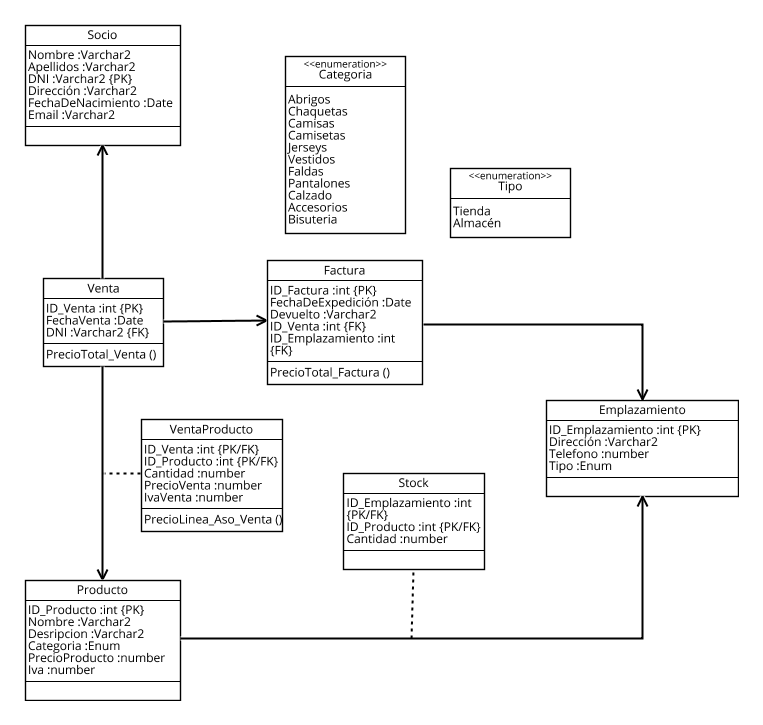
\includegraphics[width=\linewidth]{images/3FN/3FN-venta.png}
	\caption{3FN Venta}
\end{figure}

\subsection{3FN Traspaso - Pedido}

\begin{itemize}
	\item [Proveedor] Tiene una relación 1 - n con Pedido, proveedor mantiene todos sus atributos de manera directa en la 3FN y añade un ID\_PROVEEDOR como primary key.
	\item [Emplazamiento] Tiene una relación 1 - n con Pedido, pedido mantiene todos sus atributos de manera directa  en la 3FN, añade un ID\_PEDIDO como primary key y un
	ID\_PROVEEDOR como foreign key debido a la relación con Proveedor.
	\item [Pedido] Tiene una relación n - m con Producto, se crea una tabla intermedia debido a esta relación que es la tabla Asociación Pedido-Producto, con los
	siguientes atributos: cantidad, precioCompra, ivaCompra. Además tiene ID\_PEDIDO y ID\_PRODUCTO como primary keys y foreigns keys, estas claves son provocadas
	por la relación n - m entre Pedido y Producto.
	\item[Albarán] Tiene una relación 1 - 0..1 con Pedido, albarán mantiene todos sus atributos de manera directa en la 3FN y añade un ID\_ALBARAN como primary key.
	\item[Emplazamiento] Tiene una relación 1 - m bidireccional con Traspaso, traspaso mantiene todos sus atributos de manera directa en la 3FN y añade un ID\_TRASPASO.
	
	\item[Emplazamiento] Tiene una relación 1 - m bidireccional con Solicitud-Trapaso, solicitud-traspaso mantiene todos sus atributos de manera directa en la 3FN
	y añade un ID\_Solicitud.
	\item[Traspaso] Tiene una relación n - m con Producto, esto da lugar a la creación de una tabla intermedia, para poder tratas la relación n-m, con los siguientes
	atributos: cantidad, ID\_Producto(primary key y foreign key) y ID\_Traspaso(primary key y foreign key). Estas claves son provocadas por la relación n - m
	entre Traspaso y Producto.
	\item[Solicitud-Trapaso] Tiene una relación n - m con Producto, esto da lugar a la creación de una tabla intermedia, para poder tratas la relación n-m, con los siguientes
	atributos: cantidad, ID\_Producto(primary key y foreign key) y ID\_SOLICITUD(primary key y foreign key). Estas claves son provocadas por la relación n - m
	entre Solicitud-Traspaso y Producto.
	
\end{itemize}

\begin{figure}[H]
	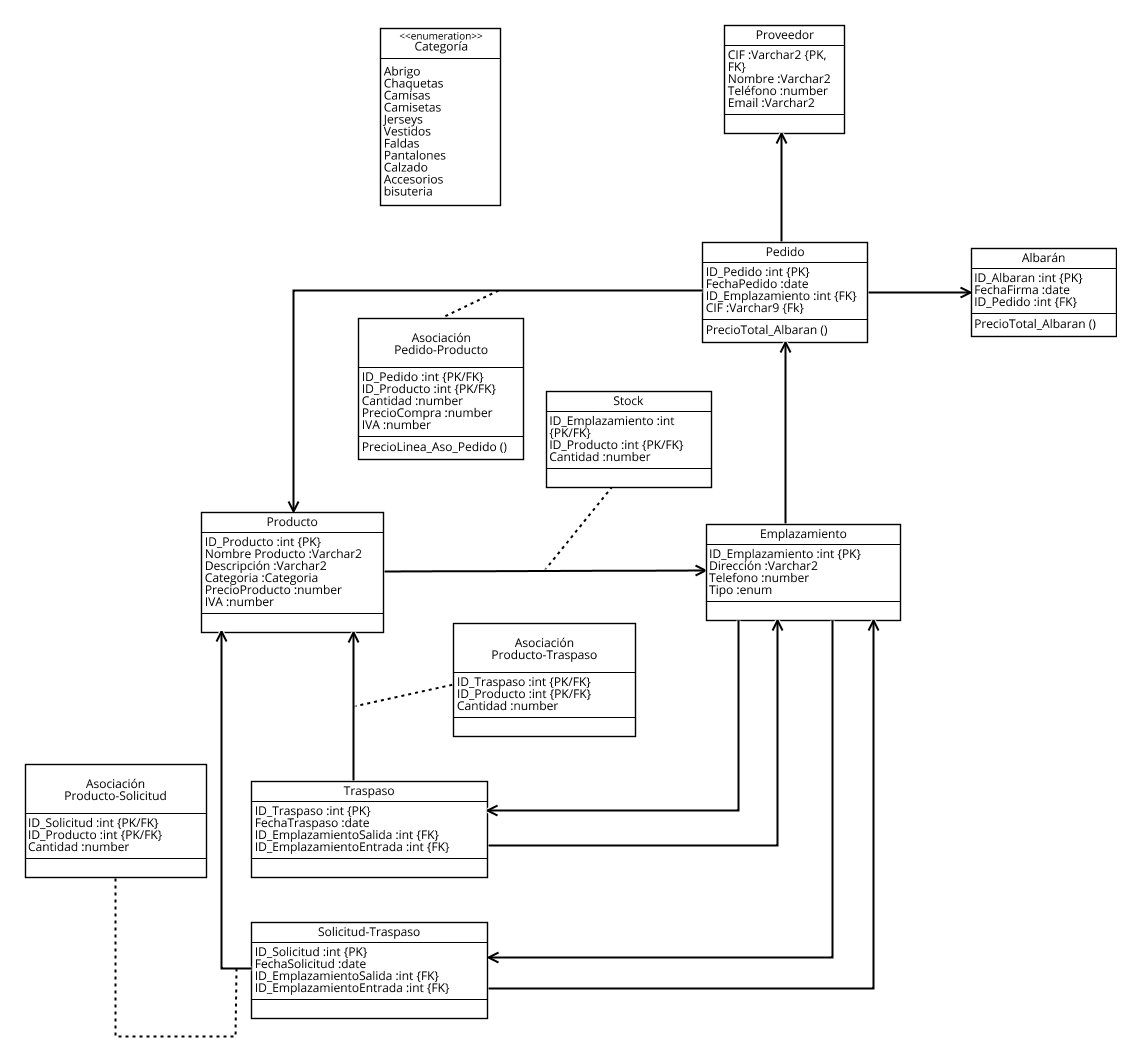
\includegraphics[width=\linewidth]{images/3FN/3FN-traspaso-pedido.png}
	\caption{3FN Traspaso - Pedido}
\end{figure}

\section{Código SQL de la base de datos}

\subsection{Tablas}
\lstinputlisting[language=SQL]{sql/tablas.sql}<

\subsection{Funciones y Procedures}
\lstinputlisting[language=SQL]{sql/funciones_y_procedures.sql}

\subsection{Triggers}

\lstinputlisting[language=SQL]{sql/triggers.sql}

\subsection{Pruebas}
\lstinputlisting[language=SQL]{sql/pruebas.sql}

\section{Apéndice}
\subsection{Actas de reunión}

\includegraphics[height=16cm, center]{images/acta1.jpg} \newpage

\includegraphics[height=16cm, center]{images/acta2.jpg}
\end{document}